\documentclass[11pt,a4paper]{article}
\usepackage[T1]{fontenc}
\usepackage[margin=2.3cm]{geometry}
\usepackage{amsmath,amssymb}
\usepackage{graphicx}
\usepackage[dvipsnames]{xcolor}
\usepackage{enumitem}
\usepackage[colorlinks=true,linkcolor=blue,urlcolor=blue]{hyperref}
\setlength{\parskip}{0.6em}
\setlength{\parindent}{0pt}
\begin{document}

\begin{center}{\LARGE\bfseries openoscillator}\\[0.4em]{\large Tune a pendulum or a spring to the exact period you want, in three sessions.}\\[0.2em]\small PAN IIT OSS explainer \textbullet{} secondary school to diploma / undergraduate (levels 3-5)\end{center}

\section*{Why this exists}
Pendulums, springs, car suspensions, bridges and radio tuners all share one idea: a restoring force that pulls a system back to rest. This explainer follows that idea from a simple period formula to a numerical simulation and resonance, using only algebra and a little programming, so you can build it yourself.

\section*{The end goal}
Tune a spring-mass or pendulum to a target period with damping. The end goal is tuning an oscillator: choosing a length, a stiffness and a damping to reach a target period or frequency, and checking the answer by simulation. The same mathematics sets the frequency of clocks, phone vibration sensors and building vibration absorbers.

\section*{How the three sessions build up}
\begin{enumerate}[nosep]
\item \textbf{Session 1: Things that swing: period, amplitude and frequency} (Level 1, conceptual interactive model, 60 min).
\item \textbf{Session 2: Simple harmonic motion, energy and damping} (Level 2, mathematical engineering model, 75 min).
\item \textbf{Session 3: The real pendulum: RK4, validation and resonance} (Level 3, simulation and validation, 90 min).
\end{enumerate}

\section{Session 1: Things that swing: period, amplitude and frequency}

\subsection*{A. Real-world problem}
A playground swing, a grandfather clock and the bouncing of a bike seat all repeat a motion again and again. How long does one swing take? How far does it go? Does a heavier child swing faster? These are questions about the period, the amplitude and the frequency of a swing, and a short graph of position against time answers all three.

\subsection*{B. Concept and theory}
A swing that repeats is called an oscillation. One full back-and-forth takes the period T (seconds). The number of swings per second is the frequency f = 1 / T (hertz, Hz). The largest distance from the middle is the amplitude A. For small swings, the period of a mass m on a spring of stiffness k is T = 2 pi sqrt(m / k), and the period of a pendulum of length L is T = 2 pi sqrt(L / g), where g = 9.81 m/s\textasciicircum{}2. The pendulum period contains no mass and no amplitude: the pull of gravity and the inertia of the bob are both proportional to the mass, so the mass cancels. The position follows a cosine wave, x(t) = A cos(2 pi t / T), if the swing starts at its largest displacement.

\begin{itemize}[nosep]
\item T: period: time for one full swing (s)
\item f: frequency: swings per second, 1 / T (Hz)
\item A: amplitude: largest displacement from the middle (m)
\item m: mass hanging on the spring (kg)
\item k: spring stiffness: force per metre of stretch (N/m)
\item L: pendulum length from pivot to the centre of the bob (m)
\item g: gravitational acceleration (m/s\textasciicircum{}2)
\end{itemize}

\begin{equation*}
T = 2\pi\sqrt{\frac{m}{k}}\qquad T = 2\pi\sqrt{\frac{L}{g}}
\end{equation*}

\begin{equation*}
f = \frac{1}{T}
\end{equation*}

\begin{equation*}
x(t) = A\cos\!\left(\frac{2\pi t}{T}\right)
\end{equation*}

\begin{center}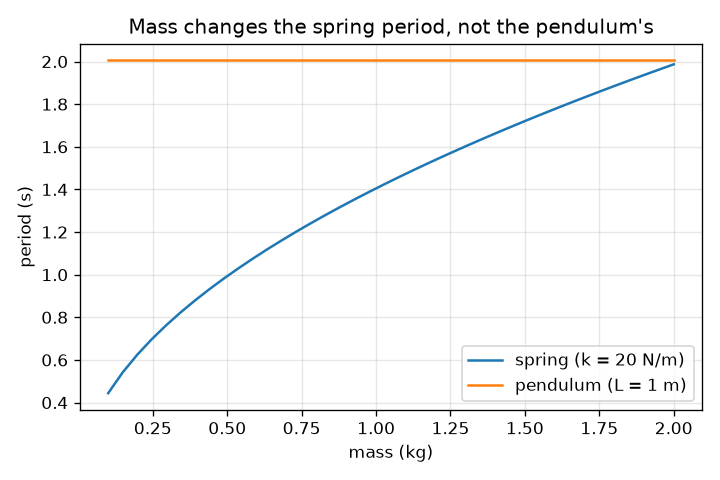
\includegraphics[width=0.85\linewidth]{figures/s01_mass_test.png}\\\small Period against mass: it grows for the spring and stays flat for the pendulum.\end{center}

\subsection*{E. Worked example}
A 0.5 kg mass hangs on a 20 N/m spring, and a 1.0 m pendulum swings next to it. Find each period and frequency, and check the pendulum with a time measurement.
\begin{enumerate}[nosep]
\item Spring: m / k = 0.5 / 20 = 0.025 s\textasciicircum{}2, sqrt = 0.1581 s, so T = 2 pi * 0.1581 = 0.993 s and f = 1 / 0.993 = 1.007 Hz.
\item Pendulum: L / g = 1.0 / 9.81 = 0.1019 s\textasciicircum{}2, sqrt = 0.3193 s, so T = 2 pi * 0.3193 = 2.006 s and f = 0.498 Hz.
\item The pendulum is about twice as slow: 2.006 / 0.993 = 2.02.
\item Check from the graph: counting upward zero crossings of the sampled spring curve, the program measures 0.9935 s, equal to the formula.
\end{enumerate}
\textbf{Answer.} Spring: T = 0.993 s, f = 1.007 Hz. Pendulum: T = 2.006 s, f = 0.498 Hz.

\subsection*{F. Questions}
\begin{enumerate}[nosep]
\item \textbf{Conceptual.} A heavy bob and a light bob hang from strings of the same length. Which one has the longer period for small swings? Explain why the mass does not appear in T = 2 pi sqrt(L / g), and why it does appear for a spring.
\item \textbf{Numerical.} Find the period and frequency of a pendulum of length 0.25 m. By what factor does the period change if the length is made four times as long?
\item \textbf{Graph and simulation interpretation.} On the graph, the spring wave (T = 0.99 s) starts at a crest at t = 0. At about what time does it first cross zero, and how many full swings does the pendulum (T = 2.01 s) make in 6 s?
\item \textbf{Design and optimisation challenge.} Design: choose a pendulum length so that it swings in step with a 2.0 kg mass on a 20 N/m spring. State the period and say whether the answer is practical for a classroom.
\end{enumerate}

\section{Session 2: Simple harmonic motion, energy and damping}

\subsection*{A. Real-world problem}
A clock must tick once every second. A phone sensor on a spring must bounce at a chosen rate. A car must stop bouncing after one or two swings, not twenty. In each case you must choose a length, a stiffness or a damping value, and that needs equations with the right units. Can you find the length of a pendulum that makes a 1 second tick, and the damper strength that makes a spring settle in about 3 seconds?

\subsection*{B. Concept and theory}
A spring pulls back with force F = -k x. Newton's second law, m x'' = -k x, says the acceleration x'' (the rate of change of the velocity) is proportional to the displacement and points back towards the middle. The solution is x(t) = A cos(w t) with the angular frequency w = sqrt(k / m) in rad/s, and the period is T = 2 pi / w. A small-angle pendulum has the same form with w = sqrt(g / L). This is called simple harmonic motion. The kinetic energy KE = (1/2) m v\textasciicircum{}2 and the spring energy PE = (1/2) k x\textasciicircum{}2 trade places, and their sum stays (1/2) k A\textasciicircum{}2. A damping force -b v removes energy at the rate b v\textasciicircum{}2. With the decay rate gamma = b / (2 m): if gamma \textless{} w0 (damping ratio zeta = b / (2 sqrt(k m)) below 1) the motion is underdamped: it still swings, with the slightly slower angular frequency wd = sqrt(w0\textasciicircum{}2 - gamma\textasciicircum{}2), inside an envelope that falls like exp(-b t / (2 m)). At b = 2 sqrt(k m) the motion is critically damped, the fastest return with no swing; above it, overdamped, a slow creep back. Design problems run the formulas backwards: L = g (T / 2 pi)\textasciicircum{}2 and k = m (2 pi / T)\textasciicircum{}2.

\begin{itemize}[nosep]
\item x: displacement from the rest position (m)
\item w0: undamped angular frequency sqrt(k / m) (rad/s)
\item b: damping coefficient: force per unit velocity (kg/s)
\item gamma: decay rate b / (2 m) (1/s)
\item zeta: damping ratio b / (2 sqrt(k m)), 1 means critical (no unit)
\item wd: damped angular frequency sqrt(w0\textasciicircum{}2 - gamma\textasciicircum{}2) (rad/s)
\item KE, PE: kinetic and spring potential energy (J)
\end{itemize}

\begin{equation*}
m\ddot x + b\dot x + kx = 0
\end{equation*}

\begin{equation*}
x(t) = A\cos(\omega t),\qquad \omega=\sqrt{k/m},\qquad T=2\pi\sqrt{m/k},\qquad T=2\pi\sqrt{L/g}
\end{equation*}

\begin{equation*}
E = \tfrac12 m v^2 + \tfrac12 k x^2 = \tfrac12 kA^2\quad(\text{no damping})
\end{equation*}

\begin{equation*}
x(t)\approx A\,e^{-bt/2m}\cos(\omega_d t),\qquad \omega_d=\sqrt{\frac{k}{m}-\Big(\frac{b}{2m}\Big)^2}
\end{equation*}

\begin{equation*}
b_{\text{crit}} = 2\sqrt{km},\qquad \zeta=\frac{b}{2\sqrt{km}},\qquad L=g\Big(\frac{T}{2\pi}\Big)^2
\end{equation*}

\begin{center}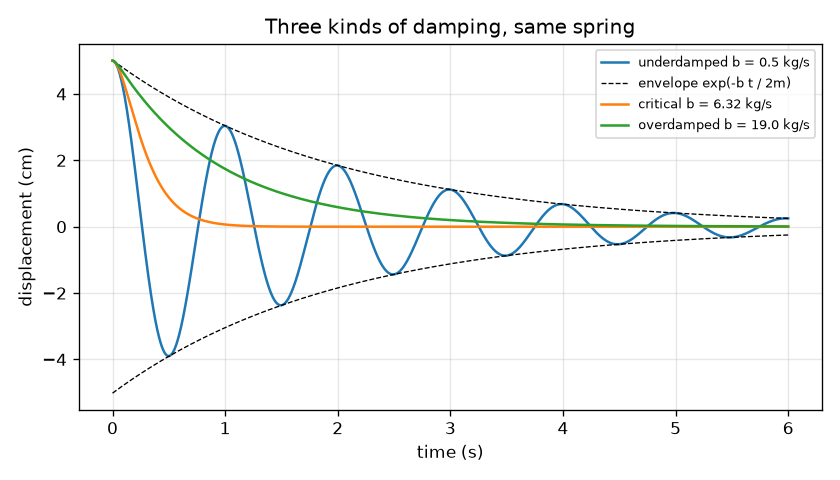
\includegraphics[width=0.85\linewidth]{figures/s02_damping_kinds.png}\\\small Same spring, three dampings: underdamped with its envelope, critical and overdamped.\end{center}

\subsection*{E. Worked example}
A 0.50 kg mass on a spring must swing with a period of 1.0 s. Find k. Then add damping b = 0.5 kg/s and find the damped period, the damping ratio and what fraction of the swing is left after 5 s. Finally find the length of the 'seconds pendulum' with a full period of 2 s.
\begin{enumerate}[nosep]
\item w = 2 pi / T = 6.283 rad/s, so k = m w\textasciicircum{}2 = 0.50 * 39.48 = 19.74 N/m.
\item Damping b = 0.5 kg/s: gamma = b / (2 m) = 0.5 / 1.0 = 0.5 1/s. Then wd = sqrt(39.48 - 0.25) = 6.263 rad/s and the damped period is 2 pi / 6.263 = 1.0032 s (a 0.3 percent change from 1.0 s).
\item Critical damping is 2 sqrt(k m) = 2 sqrt(19.74 * 0.5) = 6.283 kg/s, so zeta = 0.5 / 6.283 = 0.080: strongly underdamped.
\item After 5 s the envelope is exp(-gamma * 5) = exp(-2.5) = 0.082, or 8.2 percent of the start. Its time constant is 2 m / b = 2.0 s.
\item Seconds pendulum: L = g (T / 2 pi)\textasciicircum{}2 = 9.81 * (2 / 6.283)\textasciicircum{}2 = 9.81 * 0.10132 = 0.994 m. For a 1 s full period, L = 0.2485 m.
\end{enumerate}
\textbf{Answer.} k = 19.74 N/m; damped period 1.003 s, zeta = 0.080, 8.2 percent of the swing left after 5 s; the seconds pendulum (T = 2 s) needs L = 0.994 m.

\subsection*{F. Questions}
\begin{enumerate}[nosep]
\item \textbf{Conceptual.} With no damping, the total energy stays constant while kinetic and potential energy change. Where is the energy at the end of the swing and where at the middle? When damping is switched on, where does the lost energy go?
\item \textbf{Numerical.} A sensor of mass 0.20 kg must oscillate at 2 Hz on a spring. What stiffness is needed? What pendulum length would give a period of 1.5 s?
\item \textbf{Graph and simulation interpretation.} On the displacement graph for m = 0.5 kg, k = 20 N/m, b = 0.5 kg/s, read the time at which the envelope has fallen to half of its starting value, and compare with the formula.
\item \textbf{Design and optimisation challenge.} Design: for the m = 0.5 kg, k = 20 N/m spring, choose a damping b so that the swing is at most 5 percent of its start after 3 s. Compare with critical damping and say what you would pick for a car suspension.
\end{enumerate}

\section{Session 3: The real pendulum: RK4, validation and resonance}

\subsection*{A. Real-world problem}
The formula T = 2 pi sqrt(L / g) is a small-angle approximation: the true restoring force on a pendulum is proportional to sin(theta), not theta. A clock whose pendulum swings too far runs slow. There is no neat formula for the whole motion, so we simulate it step by step, and then we must prove that the simulation can be trusted. We also push an oscillator with a periodic force and ask: at what frequency does a small push give the largest swing, and how sharp is that peak?

\subsection*{B. Concept and theory}
With angle theta and angular velocity omega, the damped pendulum obeys theta' = omega and omega' = -(g/L) sin(theta) - c omega. We advance it in small time steps dt. Explicit Euler uses only the slope at the start of each step, and its error is proportional to dt; RK4 combines four slopes (start, two middle estimates, end) and its error shrinks like dt\textasciicircum{}4. The exact period of the undamped pendulum released from rest at theta0 is T = T0 (2/pi) K(k) with k = sin(theta0/2) and K the complete elliptic integral of the first kind; this equals T0 / AGM(1, cos(theta0/2)), where the arithmetic-geometric mean AGM is found by repeatedly replacing (a, b) by their arithmetic and geometric means. For moderate angles, T = T0 (1 + theta0\textasciicircum{}2/16 + 11 theta0\textasciicircum{}4/3072 + ...). The simulation is validated by three tests: it must match the small-angle cosine at tiny amplitude, keep the energy constant when c = 0, and shrink successive maxima by exp(-c Td / 2) when damped. For a driven linear oscillator x'' + 2 zeta w0 x' + w0\textasciicircum{}2 x = F cos(Omega t) the steady amplitude is F / sqrt((w0\textasciicircum{}2 - Omega\textasciicircum{}2)\textasciicircum{}2 + (2 zeta w0 Omega)\textasciicircum{}2), which peaks near Omega = w0 at about 1 / (2 zeta) times the static displacement F / w0\textasciicircum{}2. That ratio is the quality factor Q.

\begin{itemize}[nosep]
\item theta: angle from the downward vertical (rad (degrees in graphs))
\item omega: angular velocity theta' (rad/s)
\item c: damping rate of the pendulum (1/s)
\item dt: time step of the solver (s)
\item T0: small-angle period 2 pi sqrt(L / g) (s)
\item F: driving force per unit mass (m/s\textasciicircum{}2)
\item Omega: driving angular frequency (rad/s)
\item Q: quality factor 1 / (2 zeta): peak height over static displacement (no unit)
\end{itemize}

\begin{equation*}
\ddot\theta = -\frac{g}{L}\sin\theta - c\,\dot\theta
\end{equation*}

\begin{equation*}
y_{n+1} = y_n + \frac{\Delta t}{6}\left(k_1 + 2k_2 + 2k_3 + k_4\right)
\end{equation*}

\begin{equation*}
T = T_0\,\frac{2}{\pi}K(k)=\frac{T_0}{\mathrm{AGM}\big(1,\cos(\theta_0/2)\big)},\quad k=\sin\frac{\theta_0}{2}
\end{equation*}

\begin{equation*}
T \approx T_0\left(1+\frac{\theta_0^2}{16}+\frac{11\,\theta_0^4}{3072}\right)
\end{equation*}

\begin{equation*}
A(\Omega)=\frac{F}{\sqrt{(\omega_0^2-\Omega^2)^2+(2\zeta\omega_0\Omega)^2}},\qquad Q=\frac{1}{2\zeta}
\end{equation*}

\begin{center}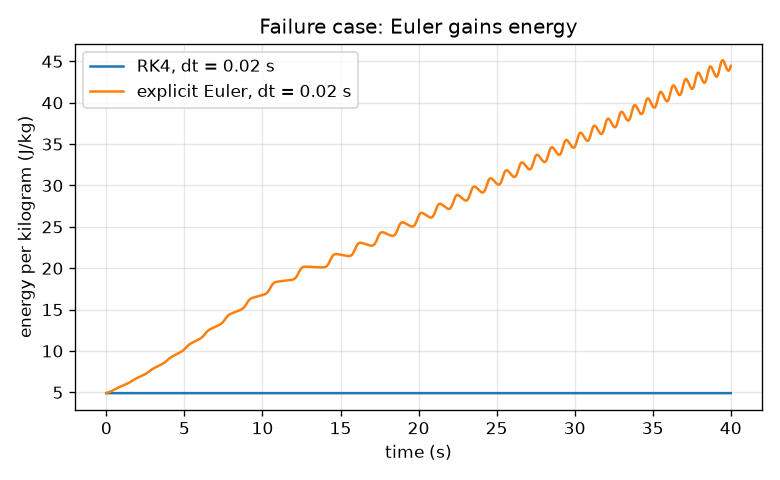
\includegraphics[width=0.85\linewidth]{figures/s03_euler_failure.png}\\\small Failure case: explicit Euler gains energy, RK4 keeps it constant.\end{center}

\subsection*{E. Worked example}
A 1.0 m pendulum is released from 40 degrees. Find its exact period and compare it with the small-angle formula and the series. At which amplitude is the small-angle formula wrong by 5 percent? Validate the simulation, and show what Euler does.
\begin{enumerate}[nosep]
\item T0 = 2 pi sqrt(1.0 / 9.81) = 2.0061 s.
\item Exact (AGM): cos(20 degrees) = 0.9397, AGM(1, 0.9397) = 0.9697, so T = 2.0061 / 0.9697 = 2.0689 s. The RK4 simulation (dt = 0.005 s) measures 2.0689 s.
\item Series: theta0 = 0.6981 rad, theta0\textasciicircum{}2/16 = 0.0305, 11 theta0\textasciicircum{}4/3072 = 0.00085, so T = 2.0061 * 1.0314 = 2.0689 s. The one-term series gives 2.0672 s.
\item The small-angle formula is low by (2.0689 - 2.0061) / 2.0689 = 3.04 percent at 40 degrees. It is 1 percent low at 22.9 degrees and 5 percent low at 51.3 degrees (bisection on the exact period). So about 40 degrees is already a 3 percent error, not yet 5.
\item Validation: for a 0.5 degree swing the largest difference between RK4 and 0.5 deg * cos(w t) over 10 s is about 1e-6 rad. Over 20 s at 60 degrees the energy drift is -5.4e-10 for RK4 (dt = 0.005 s) and +110 percent for explicit Euler with the same step. With damping c = 0.4 1/s, successive maxima ratio is 0.6689, against exp(-c Td / 2) = 0.6690.
\item Resonance: for zeta = 0.05, w0 = 2 pi rad/s, the RK4 amplitude peak is 10.00 times the static value and the half-power width gives Q = 9.90, against the formula 1 / (2 zeta) = 10.
\end{enumerate}
\textbf{Answer.} T(40 degrees) = 2.0689 s, 3.04 percent above the small-angle 2.0061 s; the formula is 5 percent low at 51.3 degrees. RK4 passes the analytic, energy and envelope tests; Euler gains energy; Q = 10 for zeta = 0.05.

\subsection*{F. Questions}
\begin{enumerate}[nosep]
\item \textbf{Conceptual.} Why does the period of a real pendulum increase with amplitude, while a mass on an ideal spring has a period that does not?
\item \textbf{Numerical.} A clock with a pendulum tuned to a 2.000 s period for small swings is driven so that it swings 30 degrees. By what percent is the period longer and how many seconds per day does the clock lose?
\item \textbf{Graph and simulation interpretation.} On the resonance curve for zeta = 0.05 the peak is at Omega / w0 = 0.9975 with height 10. Predict the peak height if the damping doubles to zeta = 0.1, and say what happens to the width of the peak.
\item \textbf{Design and optimisation challenge.} Design: you need the pendulum energy to stay within 1 percent over 20 s (60 degrees). Compare RK4 with explicit Euler: which time step and how many steps does each need? Justify.
\end{enumerate}

\section{Real-world mini-project}
\textbf{Tune a spring so a phone sensor bounces at 2 Hz.} A phone (0.170 kg) is strapped to a coil spring of mass 0.030 kg and bounces up and down, measured by its accelerometer. Only stock springs of 10, 15, 20, 25, 30, 40 and 60 N/m are available, and the setup has a damping of about 0.2 kg/s. The target frequency is 2.0 Hz. Use \texttt{tune\_spring} from Session 3 to pick the best spring, then \texttt{ballast\_for\_target} to find how much extra mass (coins taped to the strap) brings the damped frequency to 2.0 Hz, and confirm with \texttt{simulate\_spring\_mass}. This is a simplified model: a real mount adds strap flexing, air drag and sideways wobble, so treat the result as a starting point and measure.

\section{The path ahead}
\begin{enumerate}[nosep]
\item \textbf{Session 4: Chaos in the driven pendulum.} A driven version of the RK4 pendulum with phase portrait and a pair of nearby starting angles.
\item \textbf{Session 5: Fit a phone recording.} A fitting function for a damped cosine and a synthetic 'accelerometer recording' to test it.
\item \textbf{Session 6: Coupled pendulums and beats.} Two identical pendulums joined by a weak spring, simulated with RK4.
\item \textbf{Session 7: Pumping a swing: parametric resonance.} A small-angle pendulum whose length is modulated in time.
\item \textbf{Session 8: Hardening spring: the resonance curve bends.} A driven oscillator with a cubic spring term, swept up and then down in frequency.
\end{enumerate}

\section{Answers and hints}

\subsection*{Session 1}
\begin{enumerate}[nosep]
\item \textbf{Conceptual.} Hint: Compare how the restoring force and the inertia depend on the mass in each case. Solution: They have the same period. The pull of gravity along the swing is proportional to the mass, and so is the inertia (resistance to acceleration), so the mass cancels. For a spring, the restoring force k x does not grow with the mass, but the inertia does, so a larger mass accelerates less and the swing is slower: T grows like sqrt(m).
\item \textbf{Numerical.} Hint: T = 2 pi sqrt(L / g) with g = 9.81 m/s\textasciicircum{}2. A factor of 4 inside a square root becomes a factor of 2. Solution: L / g = 0.25 / 9.81 = 0.02548 s\textasciicircum{}2, sqrt = 0.1596 s, T = 2 pi * 0.1596 = 1.003 s and f = 1 / 1.003 = 0.997 Hz. Four times the length (1.0 m) gives T = 2.006 s, twice as long. Sanity check: a 25 cm pendulum is a short one, about one swing per second, which feels right.
\item \textbf{Graph and simulation interpretation.} Hint: A cosine crosses zero a quarter of a period after a crest. Solution: A quarter period is 0.993 / 4 = 0.248 s, so the spring wave first crosses zero at about 0.25 s, going downward. The pendulum makes 6 / 2.006 = 2.99, about 3 full swings in 6 s (it is nearly back at a crest at t = 6 s).
\item \textbf{Design and optimisation challenge.} Hint: First find the spring period, then solve T = 2 pi sqrt(L / g) for L: L = g (T / 2 pi)\textasciicircum{}2. Solution: Spring: T = 2 pi sqrt(2.0 / 20) = 1.987 s. Then L = 9.81 * (1.987 / 6.283)\textasciicircum{}2 = 9.81 * 0.1000 = 0.981 m. A string of about 1 m is easy to hang from a door frame, so it is practical. Trade-off: the match is only as good as the length and spring constant you can measure, and a small mismatch of 1 percent in L is 0.5 percent in T. Assumption: small swings.
\end{enumerate}

\subsection*{Session 2}
\begin{enumerate}[nosep]
\item \textbf{Conceptual.} Hint: Think about the speed at the ends and at the middle of a swing. Solution: At the ends of the swing the mass is momentarily at rest, so all the energy is stored in the spring (or, for the pendulum, in height): PE = (1/2) k A\textasciicircum{}2 and KE = 0. At the middle the spring is relaxed and the speed is largest, so all the energy is kinetic. With damping, energy is removed at the rate b v\textasciicircum{}2 and becomes heat in the damper and the air; the total falls, fastest when the speed is greatest.
\item \textbf{Numerical.} Hint: T = 1 / f = 0.5 s, then k = m (2 pi / T)\textasciicircum{}2. For the pendulum, L = g (T / 2 pi)\textasciicircum{}2. Solution: T = 0.5 s, so w = 2 pi / 0.5 = 12.57 rad/s and k = 0.20 * 157.9 = 31.58 N/m. Pendulum: L = 9.81 * (1.5 / 6.283)\textasciicircum{}2 = 9.81 * 0.05699 = 0.559 m. Sanity check: a 0.2 kg phone on a spring of 30 N/m is about right for a quick bounce, and a bit more than half a metre of string for a 1.5 s swing feels plausible.
\item \textbf{Graph and simulation interpretation.} Hint: The envelope is A exp(-b t / (2 m)); set it equal to A / 2. Solution: exp(-b t / 2m) = 0.5 gives t = 2 m ln 2 / b = 2 * 0.5 * 0.693 / 0.5 = 1.386 s. On the graph the dashed envelope crosses half height at about 1.4 s, which is a little more than one swing (T = 0.997 s). After a second half-time (2.77 s) a quarter is left.
\item \textbf{Design and optimisation challenge.} Hint: Require exp(-b * 3 / (2 * 0.5)) \textless{}= 0.05, and compare with the critical value 2 sqrt(k m). Solution: exp(-3 b) \textless{}= 0.05 needs b \textgreater{}= ln(20) / 3 = 0.9986, so b = 1.0 kg/s works: exp(-3) = 0.0498, 4.98 percent left, with zeta = 0.158 (it still swings about three times). Critical damping, b = 6.32 kg/s, would leave about 1e-7 of the start after 3 s and no swing at all, but it needs a much stronger damper, and an overdamped system is slow to follow bumps. Cars choose zeta between about 0.2 and 0.7 as a compromise: comfortable, but settling in one or two swings.
\end{enumerate}

\subsection*{Session 3}
\begin{enumerate}[nosep]
\item \textbf{Conceptual.} Hint: Compare the restoring force sin(theta) with theta, and a spring's force k x. Solution: For a spring the restoring force is exactly proportional to the displacement, so the oscillation is simple harmonic and its period is independent of amplitude. For a pendulum the restoring force goes as sin(theta), which is smaller than theta at large angles (sin 60 degrees = 0.866 against 1.047 rad), so the pull-back is weaker than the small-angle model assumes, the acceleration is smaller and each swing takes longer.
\item \textbf{Numerical.} Hint: Use the series T = T0 (1 + theta0\textasciicircum{}2 / 16 + 11 theta0\textasciicircum{}4 / 3072) with theta0 in radians, then compare tick counts over 86400 s. Solution: theta0 = 0.5236 rad, theta0\textasciicircum{}2/16 = 0.01713, 11 theta0\textasciicircum{}4/3072 = 0.00027, so T = 2.000 * 1.0174 = 2.035 s (the exact value is 1.7409 percent larger). The clock ticks 1 / 1.0174 as often, so it loses 86400 * (1 - 1 / 1.0174) = 1478 s per day, about 24.6 minutes. Hence real clocks use a small amplitude of about 3 to 4 degrees.
\item \textbf{Graph and simulation interpretation.} Hint: Q = 1 / (2 zeta); the peak width at 1/sqrt(2) of the height is about w0 / Q. Solution: Q = 1 / (2 * 0.1) = 5 (the precise peak is 5.03 times the static displacement). The peak is half as high, and its width is about twice as large (w0 / Q goes from 0.1 w0 to 0.2 w0), so the oscillator responds less strongly but over a wider range of driving frequencies. Low damping means a tall, narrow, selective resonance (a radio tuner); high damping a low broad one (a car suspension).
\item \textbf{Design and optimisation challenge.} Hint: From the lesson output, RK4 drift at dt = 0.05 s is -5.7e-5; Euler at dt = 0.005 s is +110 percent. Euler's energy grows like exp(w\textasciicircum{}2 dt T). Solution: RK4 with dt = 0.05 s has a drift of 5.7e-5 (0.006 percent), far inside 1 percent, with only 400 steps of four slope evaluations each, 1600 evaluations. Explicit Euler at 10 times smaller steps (dt = 0.005 s, 4000 steps) still gains 110 percent. Since Euler's energy grows like exp(w\textasciicircum{}2 dt T) with w\textasciicircum{}2 = 9.81 and T = 20 s, a 1 percent limit needs dt of about 5e-5 s, a few hundred thousand steps (an estimate from the growth formula). RK4 is cheaper by two or three orders of magnitude here. Trade-off: RK4 does not conserve energy exactly either; over very long runs a symplectic method may be preferred.
\end{enumerate}

\section{How to join}
Read \texttt{CONTRIBUTING.md} in the repository, then pick an issue labelled \texttt{good first issue}. Repository: \url{https://github.com/KrunalPanchal1995/openoscillator}

\end{document}
